\section{apple}

\frame{\sectionpage}

\begin{frame}
	Now, we go the other way around. Let us assume Newton is right, and see what we get. \\
	From the fact that the force is central, we immediately get the Conservation of Angular Momentum, and are able to define a plane of motion of the two bodies.\\
\end{frame}

\begin{frame}
	The usual derivation is straightforward and lengthy (i.e. not fun), so we shall take the scenic route by considering the quantity (for any general central force, $\vb{F}=f(r)\hat{\vb{r}}$)
	\begin{align*}
		\dv{t}(\vb{p}\cross\vb{L}) &= \dot{\vb{p}}\cross \vb{L} = f(r) \hat{\bm{r}}\cross(m\vb{r}\cross \dot{\vb{r}})\\
		&= \frac{mf(r)}{r} \left (\vb{r}\cross(\vb{r}\cross\vb{\dot{r}})\right)\\
		&= \frac{mf(r)}{r} \left(r\dot{r} \vb{r} - r^2\vb{\dot{r}}\right)\\
		&= mf(r)r^2\left (\frac{\dot{r}\vb{r}}{r^2}-\frac{\vb{\dot{r}}}{r}\right )
	\end{align*}
	\begin{equation*}
		\dv{t}(\vb{p}\cross\vb{L}) = mf(r)r^2\dv{t}\left (\frac{\vb{r}}{r}\right )
	\end{equation*}
	If only $f(r)\ r^2$ were a constant of some sort. Then we could have a quantity called the Laplace-Runge-Lenz vector which would have been constant with time.
\end{frame}

\begin{frame}
	
	\onslide*<1->{We define
		\begin{equation*}
		\vb{A} = \vb{p}\cross\vb{L} - mk\hat{\vb{r}}
		\end{equation*}
		and we know that $\dot{\vb{A}} = 0$ from earlier (and $k=GMm$). 
		A very good question to ask at this point would be "What is this vector?" \\
		What is constant in the orbital motion of a planet?}
	\\[3\baselineskip]
	\onslide+<2->{The orbit.}	
\end{frame}

\begin{frame}
	\begin{figure}
		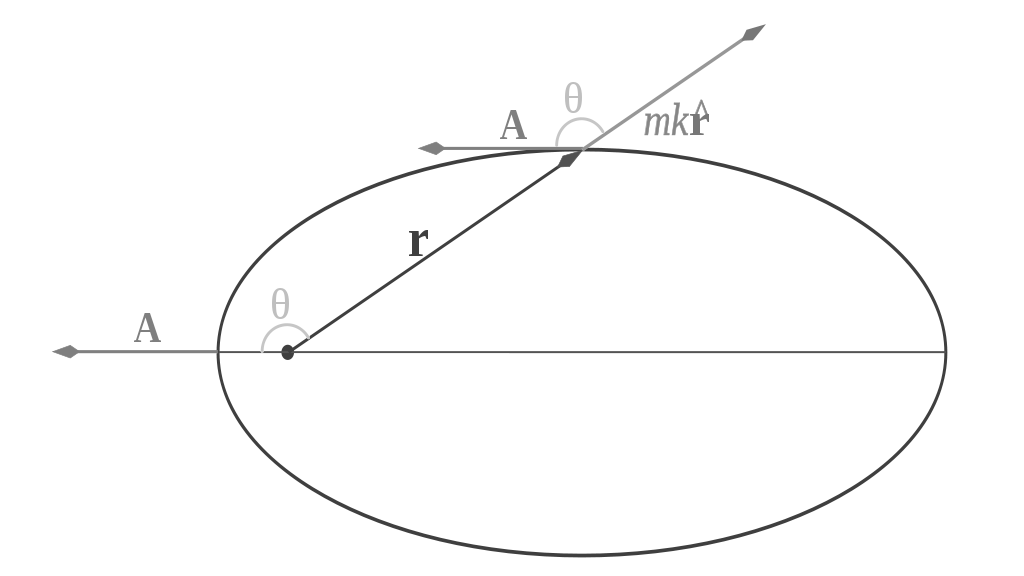
\includegraphics[width=\linewidth]{./images/LRL.png}
		\caption{\href{https://en.wikipedia.org/wiki/Laplace-Runge-Lenz\_vector}{Wikipedia}}
	\end{figure}
\end{frame}
\begin{frame}
	Since we want to know the variation of $\theta$ with $r$, we can take a dot product:
	\begin{equation*}
		\vb{A}\cdot\vb{r} = Ar \cos \theta = \vb{r}\cdot(\vb{p}\cross\vb{L}) - mkr
	\end{equation*}
	\begin{equation*}
		\vb{r}\cdot(\vb{p}\cross\vb{L})	= (\vb{r} \cross \vb{p})\cdot\vb{L} = \vb{L}\cdot\vb{L} = L^2
	\end{equation*}
	So, without any pain whatsoever, we have 
	\begin{equation*}
		r = \frac{L^2/mk}{1 + A/mk\cos\theta}
	\end{equation*}
	Note that $e = \frac{A}{mk}$, and so $\frac{\vb{A}}{mk}$ is often called the eccentricity vector.
\end{frame}

\begin{frame}
	Taking the dot product of $\vb{A}$ with itself gives the expression for energy in terms of the eccentricity
	\begin{equation*}
		A^2 = m^2k^2 + 2mEL^2
	\end{equation*}
	\begin{equation*}
		e^2 = 1 + \frac{2L^2}{mk^2}E
	\end{equation*}
	where $E = \frac{p^2}{2m} - \frac{k}{r}$
\end{frame}

